\subsection{Target Data Transfer Pipelining}
\label{sub:pipelining}

Transfer of data between host memory and the memory of an offload device such as
a GPU is a common bottleneck for heterogeneous applications.  The amount of
memory available on a given device can also vary, and the ability to adjust the
memory requirements of a given kernel based on that availability can
substantially increase the reliability of an application.  One of the most
common optimizations used to help address both of these issues is to overlap
computation with data communication to hide some of that transfer latency by
introducing multiple staging buffers and splitting the computation across them.  

Despite the fact that multiple buffers and pipelining of this kind are well
known and common patterns, the manual transformation to accomplish it requires a
significant number of changes to the source, and can easily become a source of
bugs in the transformation.  In the spirit of OpenMP, we're exploring interfaces
to allow the user to specify how their data transfers can be expressed in
connection with their offload loops iteration space.  This would allow an OpenMP
compiler to generate all of the necessary boilerplate to pipeline data transfers
for the loop or loops.  Figure~\ref{fig:pipeline} shows an example of how a
simple stencil code could be pipelined, the compiler can generate a new version
of the loop that splits the outer loop into multiple chunks that each process a
piece of the data which can then be streamed through the device without having
to pull in the entire range of the data first.

\begin{figure}
\begin{minted}{c}
void func(double *A, double *An,
          int nx, int ny, int nz) {
#pragma omp target teams distribute\
  pipeline(static)\
  map(pipeline,to:A[k-1:3][0:ny][0:nx])\
  map(pipeline,from:An[k:1][0:ny][0:nx])
for(k=1;k<nz;k++) {
  #pragma omp parallel for
  for(i=1;i<nx;i++) {
    for(j=1;j<ny;j++) {
      An[Index3D (i,     j,     k)] =
      (A[Index3D (i,     j,     k + 1)] +
       A[Index3D (i,     j,     k - 1)] +
       A[Index3D (i,     j + 1, k)] +
       A[Index3D (i,     j - 1, k)] +
       A[Index3D (i + 1, j,     k)] +
       A[Index3D (i - 1, j,     k)])* c1
     - A[Index3D (i,     j,     k)] * c0;
    }
  } 
}
}
\end{minted}
\caption{Example of a possible syntax for pipelining a stencil
loop.\label{fig:pipeline}}
\end{figure}

A working prototype of a runtime for this functionality has been
created~\cite{cui2017directive}. The performance across a number of common
kernels is presented in Figure~\ref{fig:pipeline-perf}.  There are two different
versions of the pipelining presented, the Pipelined version uses a buffer of the
same size and layout as in the naive version.  It saves no memory space, just
overlaps transfers.  The Pipelined-buffer version uses multiple smaller buffers
and transforms the accesses in the loop to decrease the memory requirements of
the kernel as well.  In some cases, particularly the 3dconv and stencil kernels,
the buffered version's greater locality actually provides better performance
than baseline. In the case of the quantum chromo-dynamics kernel however it is a
loss of about 20\% performance compared to using the full amount of memory, but
allows much larger problems to be run than would otherwise fit on the device.

\begin{figure}
  \centering
  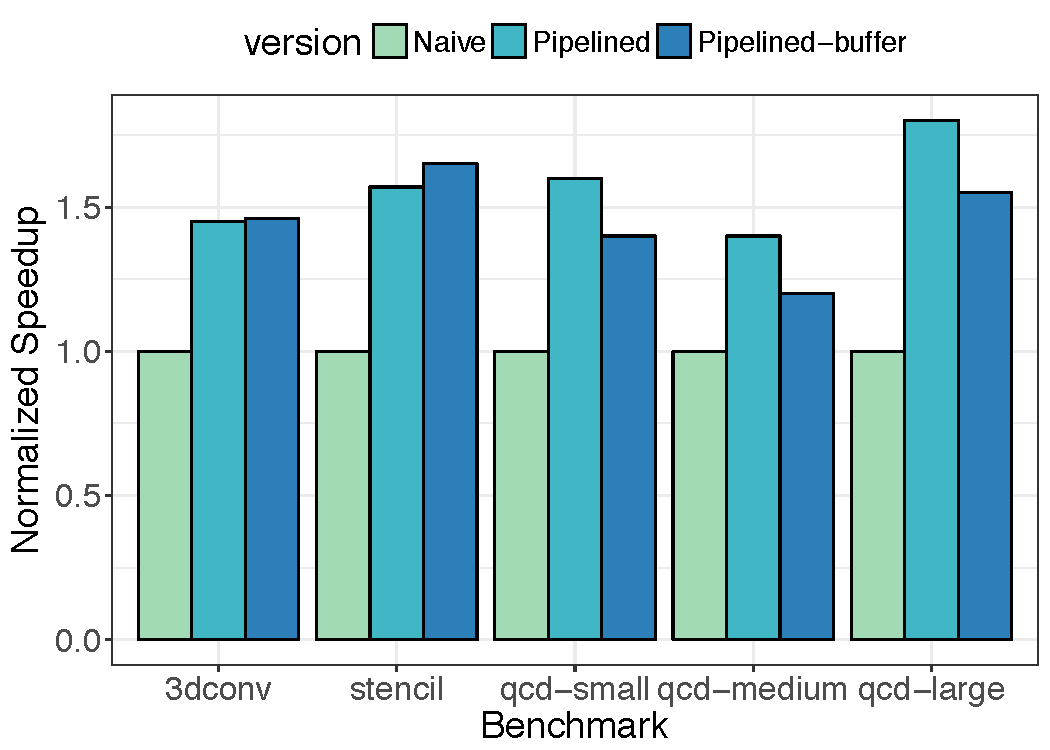
\includegraphics[width=0.5\textwidth]{pics/pipelining-perf}
  \caption{Speedup of pipelined or buffered data transfers across
  kernels.\label{fig:pipeline-perf}}
\end{figure}

